\documentclass[11pt]{article}

\usepackage[a4paper,margin=0.75in]{geometry}
\usepackage{amsmath,amssymb}
\usepackage{graphicx}
\usepackage{booktabs}
\usepackage{array}
\usepackage{float}
\usepackage{hyperref}
\usepackage{enumitem}
\usepackage{xcolor}
\usepackage{tikz}
\usetikzlibrary{positioning,arrows.meta,shapes.geometric}

\setlist{nosep}
\renewcommand{\arraystretch}{1.3}

\tikzset{
layer/.style={
draw,
rounded corners,
minimum width=2.2cm,
minimum height=0.9cm,
align=center,
fill=blue!10
},
arrow/.style={
-{Latex[length=3mm]},
thick
}
}

\begin{document}

%%%%%%%%%%%%%%%%%%%%%%%%%%%%%%%%%%%%%%%%%%%%%%%%%%%%%%%%%%%%

\begin{center}

{\Large\textbf{Shiv Nadar University Chennai}}

\vspace{3mm}

{\large\textbf{CS3807 -- Deep Learning Laboratory}}

\vspace{3mm}

{\Large\textbf{Experiment 4}}

\vspace{2mm}

{\Large\textbf{Comparative Study of Deep Convolutional Neural}}

{\Large\textbf{Network Architectures Using Transfer Learning}}

\end{center}

\vspace{5mm}

\begin{tabular}{|p{4cm}|p{8cm}|p{2cm}|}
\hline
Degree \& Branch &
B.Tech Artificial Intelligence \& Data Science &
Semester V\\
\hline
Subject Code \& Name &
CS3807 -- Deep Learning Laboratory &
AY: 2026--27\\
\hline
\end{tabular}

\vspace{4mm}
Name : Ashwin S\\
Reg no : 24011101007\\
Class : AI DS - A (batch 1)\\

%%%%%%%%%%%%%%%%%%%%%%%%%%%%%%%%%%%%%%%%%%%%%%%%%%%%%%%%%%%%

\section*{1. Objective}

The objectives of this experiment are

\begin{itemize}

\item Study the evolution of deep CNN architectures.

\item Compare LeNet-5, AlexNet, VGG16, GoogleNet and ResNet.

\item Understand transfer learning.

\item Fine tune pretrained CNN models.

\item Compare classification performance of different architectures.

\end{itemize}

%%%%%%%%%%%%%%%%%%%%%%%%%%%%%%%%%%%%%%%%%%%%%%%%%%%%%%%%%%%%

\section*{2. Learning Outcomes}

After completing this experiment students will be able to

\begin{enumerate}

\item Explain modern CNN architectures.

\item Differentiate LeNet, AlexNet, VGG16, GoogleNet and ResNet.

\item Implement transfer learning.

\item Fine tune pretrained CNN models.

\item Compare CNN architectures using performance metrics.

\end{enumerate}

%%%%%%%%%%%%%%%%%%%%%%%%%%%%%%%%%%%%%%%%%%%%%%%%%%%%%%%%%%%%

\section*{3. Introduction}

Deep Convolutional Neural Networks have become the dominant models for
computer vision applications because they automatically learn hierarchical
features from images. The evolution of CNNs has focused on improving
classification accuracy while reducing computational complexity and
training difficulties.

The progression of CNN architectures began with LeNet-5 and has evolved
through AlexNet, VGGNet, GoogleNet, and ResNet. Each architecture
introduced important innovations that significantly improved image
classification performance.

%%%%%%%%%%%%%%%%%%%%%%%%%%%%%%%%%%%%%%%%%%%%%%%%%%%%%%%%%%%%

\section*{4. Evolution of CNN Architectures}

\begin{center}

\begin{tabular}{|c|c|p{7cm}|}

\hline

Model & Year & Major Contribution\\

\hline

LeNet-5 & 1998 &
First practical convolutional neural network\\

\hline

AlexNet & 2012 &
ReLU activation, Dropout and GPU training\\

\hline

VGG16 & 2014 &
Uniform $3\times3$ convolution filters\\

\hline

GoogleNet & 2014 &
Inception modules for multi-scale feature extraction\\

\hline

ResNet & 2015 &
Residual learning using skip connections\\

\hline

\end{tabular}

\end{center}

%%%%%%%%%%%%%%%%%%%%%%%%%%%%%%%%%%%%%%%%%%%%%%%%%%%%%%%%%%%%

\section*{5. LeNet-5}

LeNet-5 was proposed by Yann LeCun in 1998 for handwritten digit
recognition. It consists of two convolution layers, two average pooling
layers and fully connected layers. It demonstrated that convolutional
networks could automatically learn image features without handcrafted
feature extraction.


Advantages

\begin{itemize}

\item Small number of parameters

\item Fast training

\item Suitable for OCR

\end{itemize}

%%%%%%%%%%%%%%%%%%%%%%%%%%%%%%%%%%%%%%%%%%%%%%%%%%%%%%%%%%%%

\section*{6. AlexNet}

AlexNet won the ImageNet Challenge in 2012 by reducing the
classification error significantly. It introduced ReLU activation,
Dropout regularization and GPU training.


Major innovations

\begin{itemize}

\item ReLU activation

\item Dropout

\item GPU implementation

\item Data augmentation

\end{itemize}

%%%%%%%%%%%%%%%%%%%%%%%%%%%%%%%%%%%%%%%%%%%%%%%%%%%%%%%%%%%%

\section*{7. VGG16}

VGG16 demonstrated that using multiple small $3\times3$ convolution
filters could outperform larger filters while increasing network depth.


Advantages

\begin{itemize}

\item Excellent feature extraction

\item Simple architecture

\item High classification accuracy

\end{itemize}

%%%%%%%%%%%%%%%%%%%%%%%%%%%%%%%%%%%%%%%%%%%%%%%%%%%%%%%%%%%%

\section*{8. Comparison of Architectures}

\begin{center}

\begin{tabular}{|l|c|c|c|}

\hline

Architecture &
Depth &
Parameters &
Main Contribution\\

\hline

LeNet-5 &
7 &
60K &
First CNN\\

AlexNet &
8 &
61M &
ReLU + Dropout\\

VGG16 &
16 &
138M &
Deep 3$\times3$ filters\\

GoogleNet &
22 &
6.8M &
Inception Modules\\

ResNet50 &
50 &
25.6M &
Residual Learning\\

\hline

\end{tabular}

\end{center}

% --------- CONTINUE WITH PART 2 ---------
%%%%%%%%%%%%%%%%%%%%%%%%%%%%%%%%%%%%%%%%%%%%%%%%%%%%%%%%%%%%
\section*{9. GoogleNet (Inception Network)}

GoogleNet, proposed by Szegedy \textit{et al.} in 2014, introduced the
\textbf{Inception Module}, which performs multiple convolution operations
in parallel using different filter sizes. Instead of using only a single
kernel size, GoogleNet simultaneously applies $1\times1$, $3\times3$,
$5\times5$ convolutions and max pooling. The outputs are concatenated to
obtain multi-scale feature representations.

The use of $1\times1$ convolutions before larger kernels reduces the
number of trainable parameters and computational complexity.


Advantages

\begin{itemize}
\item Multi-scale feature extraction.
\item Fewer parameters than VGG16.
\item High computational efficiency.
\item Better classification performance.
\end{itemize}

%%%%%%%%%%%%%%%%%%%%%%%%%%%%%%%%%%%%%%%%%%%%%%%%%%%%%%%%%%%%

\section*{10. ResNet}

Increasing CNN depth often causes the \textbf{vanishing gradient problem},
making optimization difficult. ResNet solves this issue using
\textbf{skip (residual) connections}, allowing gradients to flow directly
through the network.

Instead of learning

\[
H(x)
\]

ResNet learns

\[
F(x)=H(x)-x
\]

thus,

\[
Output = F(x)+x
\]

where

\begin{itemize}
\item $F(x)$ = Residual Mapping
\item $x$ = Identity Mapping
\end{itemize}

\begin{figure}[H]
\centering

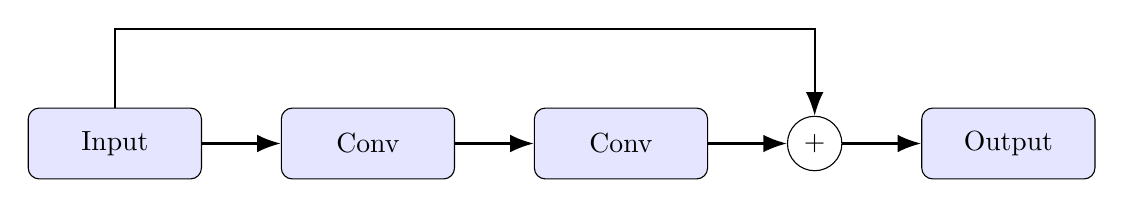
\begin{tikzpicture}[node distance=1cm]

\node[layer](input){Input};

\node[layer,right=of input](conv1){Conv};

\node[layer,right=of conv1](conv2){Conv};

\node[circle,draw,right=of conv2](add){+};

\node[layer,right=of add](output){Output};

\draw[arrow](input)--(conv1);
\draw[arrow](conv1)--(conv2);
\draw[arrow](conv2)--(add);
\draw[arrow](add)--(output);

\draw[arrow]
(input)
|-([yshift=10mm]conv2.north)
-| (add.north);

\end{tikzpicture}

\caption{Residual Block in ResNet}
\end{figure}

Advantages

\begin{itemize}
\item Eliminates vanishing gradients.
\item Enables very deep neural networks.
\item Faster convergence.
\item High ImageNet accuracy.
\end{itemize}

%%%%%%%%%%%%%%%%%%%%%%%%%%%%%%%%%%%%%%%%%%%%%%%%%%%%%%%%%%%%

\section*{11. Dilated Convolution}

Dilated convolution (also called atrous convolution) increases the
receptive field without increasing the number of parameters.

The dilation rate determines the spacing between kernel elements.

For a standard convolution,

\[
D=1
\]

For dilated convolution,

\[
D>1
\]

Example

\[
\begin{bmatrix}
1 & 0 & 2\\
0 & 3 & 0\\
4 & 0 & 5
\end{bmatrix}
\]

where zeros indicate inserted gaps.

Applications

\begin{itemize}
\item Semantic segmentation
\item Medical image analysis
\item Satellite imagery
\item Object localization
\end{itemize}

%%%%%%%%%%%%%%%%%%%%%%%%%%%%%%%%%%%%%%%%%%%%%%%%%%%%%%%%%%%%

\section*{12. Transpose Convolution}

Transpose convolution increases the spatial dimensions of feature maps.
Unlike pooling, which reduces image size, transpose convolution performs
learnable upsampling.

Applications

\begin{itemize}
\item Image Super Resolution
\item Autoencoders
\item GANs
\item Image Generation
\item Semantic Segmentation
\end{itemize}

%%%%%%%%%%%%%%%%%%%%%%%%%%%%%%%%%%%%%%%%%%%%%%%%%%%%%%%%%%%%

\section*{13. Transfer Learning}

Transfer Learning utilizes a pretrained CNN model that has already learned
general image features from a large dataset such as ImageNet.

Instead of training from scratch,

\begin{enumerate}
\item Load a pretrained model.
\item Remove the original classifier.
\item Freeze convolution layers.
\item Add new Dense layers.
\item Train the classifier.
\item Fine tune selected convolution layers.
\end{enumerate}

\begin{figure}[H]

\centering

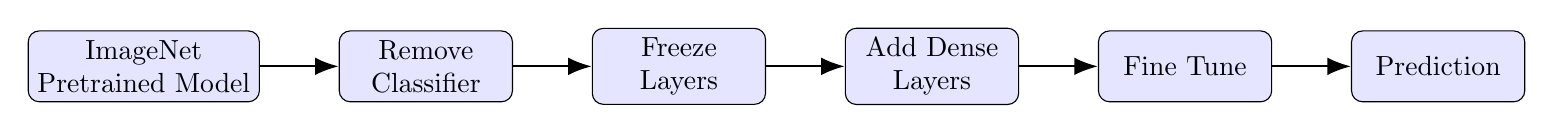
\begin{tikzpicture}[node distance=1cm]

\node[layer](a){ImageNet\\Pretrained Model};

\node[layer,right=of a](b){Remove\\Classifier};

\node[layer,right=of b](c){Freeze\\Layers};

\node[layer,right=of c](d){Add Dense\\Layers};

\node[layer,right=of d](e){Fine Tune};

\node[layer,right=of e](f){Prediction};

\foreach \x/\y in {a/b,b/c,c/d,d/e,e/f}
\draw[arrow](\x)--(\y);

\end{tikzpicture}

\caption{Transfer Learning Workflow}

\end{figure}

Advantages

\begin{itemize}
\item Faster convergence.
\item Higher accuracy on small datasets.
\item Reduced training time.
\item Lower computational cost.
\end{itemize}

%%%%%%%%%%%%%%%%%%%%%%%%%%%%%%%%%%%%%%%%%%%%%%%%%%%%%%%%%%%%

\section*{14. Dataset}

Dataset: CIFAR-10

\begin{itemize}

\item Training Images : 50,000

\item Testing Images : 10,000

\item Number of Classes : 10

\item Image Size : $32\times32\times3$ (scaled to $160\times160\times3$ )

\item Classes:
Airplane, Automobile, Bird, Cat, Deer,
Dog, Frog, Horse, Ship and Truck.

\item Dataset Source : \url{https://www.kaggle.com/datasets/pankrzysiu/cifar10-python}

\end{itemize}

%%%%%%%%%%%%%%%%%%%%%%%%%%%%%%%%%%%%%%%%%%%%%%%%%%%%%%%%%%%%
% Continue with Part 3
%%%%%%%%%%%%%%%%%%%%%%%%%%%%%%%%%%%%%%%%%%%%%%%%%%%%%%%%%%%%

\section*{15. Experimental Procedure}

\subsection*{Task 1: Dataset Preparation}

\begin{enumerate}

\item Load the CIFAR-10 dataset using TensorFlow/Keras.

\item Normalize the pixel values to the range [0,1].

\item Display ten sample images.

\item Print the dimensions of the training and testing datasets.

\end{enumerate}

NOTE : The raw CIFAR-10 pixel values were retained (not pre-scaled to [0,1]) for the models feeding into a pretrained backbone, since each backbone's own \texttt{preprocess\_input} function performs the ImageNet-specific normalization internally; pre-scaling before this step causes incorrect double normalization.

%%%%%%%%%%%%%%%%%%%%%%%%%%%%%%%%%%%%%%%%%%%%%%%%%%%%%%%%%%%%

\subsection*{Task 2: Transfer Learning}

Load any one of the following pretrained CNN models.

\begin{itemize}

\item VGG16

\item ResNet50

\item MobileNetV2

\item EfficientNetB0

\end{itemize}

Perform the following steps.

\begin{enumerate}

\item Load pretrained ImageNet weights.

\item Remove the original classification layer.

\item Freeze the convolutional base.

\item Add a Global Average Pooling layer.

\item Add a Dense layer with ReLU activation.

\item Add the output layer with Softmax activation.

\end{enumerate}

NOTE : Input images were resized from $32\times32\times3$ to $160\times160\times3$ before being passed through the VGG16 convolutional base, since pretrained ImageNet backbones expect larger spatial input dimensions than the native CIFAR-10 resolution.


%%%%%%%%%%%%%%%%%%%%%%%%%%%%%%%%%%%%%%%%%%%%%%%%%%%%%%%%%%%%

\subsection*{Task 3: Model Training}

Train the model using

\begin{center}

\begin{tabular}{|p{5cm}|p{6cm}|}

\hline

Optimizer & Adam\\

\hline

Learning Rate & 0.001\\

\hline

Batch Size & 32\\

\hline

Epochs & 20 (frozen base training)\\

\hline

Loss Function &
Categorical Cross Entropy\\

\hline

Evaluation Metric &
Accuracy\\

\hline

\end{tabular}

\end{center}

%%%%%%%%%%%%%%%%%%%%%%%%%%%%%%%%%%%%%%%%%%%%%%%%%%%%%%%%%%%%

\subsection*{Task 4: Fine Tuning}

\begin{enumerate}

\item Unfreeze the last convolution block (block5).

\item Train for another 8 epochs.

\item Compare the classification accuracy before and after fine tuning.

\end{enumerate}

%%%%%%%%%%%%%%%%%%%%%%%%%%%%%%%%%%%%%%%%%%%%%%%%%%%%%%%%%%%%

\subsection*{Task 5: Model Evaluation}

Evaluate the trained model using

\begin{itemize}

\item Accuracy

\item Precision

\item Recall

\item F1-score

\item Confusion Matrix

\item Classification Report

\end{itemize}

%%%%%%%%%%%%%%%%%%%%%%%%%%%%%%%%%%%%%%%%%%%%%%%%%%%%%%%%%%%%

\section*{16. Hyperparameter Study}

Compare the performance using different settings.

\begin{center}

\begin{tabular}{|l|l|}

\hline

Hyperparameter & Values\\

\hline

Learning Rate &
0.001, 0.0001\\

\hline

Batch Size &
16, 32, 64\\

\hline

Epochs &
3\\

\hline

Optimizer &
Adam, SGD\\

\hline

Dense Units &
128, 256\\

\hline

Frozen Layers &
All, Partial\\

\hline

\end{tabular}

\end{center}

\vspace{3mm}

Four configurations were evaluated, each trained for 3 epochs on the VGG16 transfer-learning pipeline:

\begin{center}

\begin{tabular}{|c|c|c|c|c|c|c|}

\hline

Config & LR & Batch Size & Optimizer & Dense Units & Frozen & Val. Accuracy\\

\hline

1 & 0.001 & 32 & Adam & 128 & All & 0.8533\\

\hline

2 & 0.0001 & 32 & Adam & 256 & All & 0.8478\\

\hline

3 & 0.001 & 64 & SGD & 128 & All & 0.8427\\

\hline

4 & 0.001 & 16 & Adam & 256 & Partial & 0.5451\\

\hline

\end{tabular}

\end{center}

\vspace{3mm}
Only 3 epochs were trained, considering computational time and resource constraints.

%%%%%%%%%%%%%%%%%%%%%%%%%%%%%%%%%%%%%%%%%%%%%%%%%%%%%%%%%%%%

\section*{17. Source Code}

The complete implementation, including data preprocessing, convolution and pooling experiments, model construction, training, transfer learning, evaluation, and the additional exercises, is available in the following repository :\\

    \hspace{25mm}  \url{https://github.com/Ashwin271206/dl-lab/tree/main/Lab%204}\\

The repository contains a single Google Colab notebook covering all tasks experimented in this report, along with the generated figures and outputs.

%%%%%%%%%%%%%%%%%%%%%%%%%%%%%%%%%%%%%%%%%%%%%%%%%%%%%%%%%%%%

\section*{18. Plots \& Inferences}

\begin{figure}[H]
\centering

\includegraphics[width=0.85\textwidth]{figures/01_sample_cifar10_images.png}
\caption{Sample CIFAR-10 Images}
\end{figure}

10 randomly sampled CIFAR-10 images are shown above, one label per image drawn from the ten classes. The samples confirm that the dataset was loaded and decoded correctly, with images at their native $32\times32\times3$ resolution.

\vspace{5mm}

\begin{figure}[H]
\centering

\includegraphics[width=0.75\textwidth]{figures/02_training_validation_accuracy.png}
\caption{Training and Validation Accuracy (Frozen Base, VGG16)}
\end{figure}

Training accuracy rises steadily and stabilizes near 98\% while the frozen convolutional base is used, showing the dense classifier head fitting the training data. Validation accuracy stays noticeably lower and flattens around 85--86\%, indicating a persistent generalization gap during this phase.

\vspace{5mm}

\begin{figure}[H]
\centering

\includegraphics[width=0.75\textwidth]{figures/03_training_validation_loss.png}
\caption{Training and Validation Loss (Frozen Base, VGG16)}
\end{figure}

Training loss decreases consistently across epochs, while validation loss rises after the first few epochs. This divergence between training and validation loss is a sign of overfitting when only the classifier head is being trained on frozen features.

\vspace{5mm}

\begin{figure}[H]
\centering

\includegraphics[width=\textwidth]{figures/04_combined_accuracy_loss_finetuning.png}
\caption{Combined Accuracy and Loss Across Frozen-Base and Fine-Tuning Phases}
\end{figure}

The dashed line marks the start of fine-tuning, after which validation accuracy improves markedly and validation loss drops sharply. This confirms that unfreezing the last convolutional block allows the network to adapt its ImageNet features to the CIFAR-10 domain, closing much of the earlier generalization gap.

\vspace{5mm}

\begin{figure}[H]
\centering

\includegraphics[width=0.85\textwidth]{figures/05_confusion_matrix.png}
\caption{Confusion Matrix (Fine-Tuned VGG16 Model)}
\end{figure}

The confusion matrix shows strong diagonal dominance across all ten classes, with the highest confusion occurring between visually similar categories such as cat and dog. Vehicle classes such as automobile, ship, and truck are classified with very high accuracy.

\vspace{5mm}

\begin{figure}[H]
\centering

\includegraphics[width=0.85\textwidth]{figures/06_misclassified_images.png}
\caption{Misclassified Images (Fine-Tuned VGG16 Model)}
\end{figure}

The misclassified samples largely correspond to visually ambiguous cases, such as animals in unusual poses or partially occluded objects. This is consistent with the confusion matrix, where animal classes show the most inter-class confusion.

\vspace{5mm}

\begin{figure}[H]
\centering

\includegraphics[width=0.75\textwidth]{figures/08_hyperparameter_study_accuracy.png}
\caption{Hyperparameter Study: Validation Accuracy by Configuration}
\end{figure}

Configurations 1 through 3, all using a frozen convolutional base, achieve similar validation accuracy in the 0.84--0.85 range regardless of learning rate, batch size, or optimizer choice. Configuration 4, which partially unfreezes the base with only 3 epochs of training, performs substantially worse, showing that unfreezing layers needs more epochs to converge than a frozen-base setup.

%%%%%%%%%%%%%%%%%%%%%%%%%%%%%%%%%%%%%%%%%%%%%%%%%%%%%%%%%%%%

\section*{19. Results}

\subsection*{19.1 Performance Metrics}

\begin{center}

\begin{tabular}{|p{5cm}|p{4cm}|}

\hline

Metric & Value\\

\hline

Training Accuracy & 97.572\%\\

\hline

Testing Accuracy & 91.970\%\\

\hline

Precision & 92.159\%\\

\hline

Recall & 91.970\%\\

\hline

F1-score & 92.005\%\\

\hline

Training Time & 4451.24 s\\

\hline

Total Parameters & 14,848,586\\

\hline

\end{tabular}

\end{center}

\vspace{5mm}

\subsection*{19.2 Comparison of CNN Architectures}

\begin{center}

\begin{tabular}{|l|c|c|c|}

\hline

Model &
Parameters &
Accuracy (\%) &
Training Time\\

\hline

LeNet-5 & 83,126 & 53.78 & 70.48 s\\

\hline

AlexNet & 8,576,906 & 70.61 & 290.36 s\\

\hline

VGG16 & 14,848,586 & 91.97 & 4451.24 s\\

\hline

GoogleNet (InceptionV3) & 22,329,898 & 82.83 & 597.73 s\\

\hline

ResNet50 & 24,114,826 & 86.13 & 419.78 s\\

\hline

\end{tabular}

\end{center}

%%%%%%%%%%%%%%%%%%%%%%%%%%%%%%%%%%%%%%%%%%%%%%%%%%%%%%%%%%%%


\vspace{20mm}

\section*{20. Discussion Questions}

\begin{enumerate}

\item \textbf{Why is AlexNet considered a breakthrough in deep learning?}

AlexNet was the first deep CNN to win the ImageNet Large Scale Visual Recognition Challenge by a large margin, demonstrating that deep convolutional networks could outperform traditional hand-engineered computer vision methods. It popularized ReLU activation for faster convergence, dropout for regularization, and GPU-based training for scaling to large networks and datasets, establishing the template that most modern CNNs still follow.\\

\item \textbf{Why does VGG16 use only $3\times3$ convolution filters?}

Stacking multiple $3\times3$ filters achieves the same effective receptive field as a single larger filter (e.g., two $3\times3$ layers approximate a $5\times5$ receptive field) while using fewer parameters and adding more non-linear activation steps in between. This makes the network deeper and more expressive without a proportional increase in computational cost.\\

\item \textbf{Explain the advantages of the Inception module.}

The Inception module applies multiple filter sizes ($1\times1$, $3\times3$, $5\times5$) and pooling in parallel within the same layer, allowing the network to capture features at multiple scales simultaneously. The $1\times1$ convolutions act as dimensionality reducers before the larger filters, cutting computational cost significantly while preserving representational power, resulting in a network with far fewer parameters than VGG16 for comparable depth.\\

\item \textbf{What is the purpose of residual learning?}

Residual learning reformulates each block to learn a residual function $F(x) = H(x) - x$ instead of directly learning the full mapping $H(x)$, with the output computed as $F(x) + x$. Skip connections let gradients flow directly through identity paths during backpropagation, which mitigates the vanishing gradient problem and makes it possible to train networks with far greater depth than would otherwise be feasible.\\

\item \textbf{Differentiate LeNet and ResNet.}

LeNet-5 is a shallow, 7-layer network with under 100K parameters designed for simple grayscale digit recognition using average pooling and tanh activations. ResNet50 is a 50-layer deep network with over 25M parameters that uses residual (skip) connections, batch normalization, and ReLU activations to enable stable training at much greater depth on complex, large-scale natural image datasets.\\

\item \textbf{What is Transfer Learning?}

Transfer learning is the technique of reusing a model that has already been trained on a large dataset (such as ImageNet) as the starting point for a new, related task, rather than training a new model from scratch. The pretrained convolutional layers, which have already learned general-purpose visual features like edges and textures, are retained and a new classifier head is trained on top for the target task.\\

\item \textbf{Why is fine tuning required?}

While a frozen pretrained base provides useful generic features, those features are optimized for the original dataset's domain (e.g., natural high-resolution ImageNet photos) and may not fully suit the new task's domain and image characteristics. Fine tuning unfreezes some of the later convolutional layers and continues training them at a low learning rate, allowing the network to adapt its higher-level features specifically to the target dataset and improve accuracy further.\\

\item \textbf{Explain the difference between dilated convolution and transpose convolution.}

Dilated (atrous) convolution inserts gaps between kernel elements to increase the receptive field without adding parameters or reducing spatial resolution, and is commonly used in semantic segmentation. Transpose convolution, in contrast, performs learnable upsampling to increase the spatial dimensions of a feature map, and is used in tasks like image generation, super-resolution, and autoencoder decoders.\\

\item \textbf{Why do pretrained models converge faster?}

Pretrained models start with weights that already encode useful low-level and mid-level visual features (edges, textures, shapes) learned from a large dataset, instead of starting from random initialization. This gives the optimizer a much better starting point, so fewer epochs are needed to reach good performance compared to training an equivalent network from scratch.\\

\item \textbf{Compare the computational complexity of LeNet and ResNet.}

LeNet-5 has roughly 60K parameters and 7 layers, making it extremely lightweight and fast to train even on limited hardware. ResNet50 has approximately 25.6M parameters across 50 layers with residual connections, making it far more computationally expensive to train and run inference on, though this added complexity is what enables it to model much more complex visual patterns.

\end{enumerate}

%%%%%%%%%%%%%%%%%%%%%%%%%%%%%%%%%%%%%%%%%%%%%%%%%%%%%%%%%%%%

\section*{21. Additional Exercises}

\subsection*{21.1 Implement transfer learning using VGG16}

This was implemented as the primary transfer-learning pipeline (Sections 15--19). The fine-tuned VGG16 model achieved a test accuracy of 91.97\%, with performance metrics reported in Section 19.1.

\vspace{5mm}

\subsection*{21.2 Repeat the experiment using ResNet50}

A separate transfer-learning pipeline was built using a frozen ResNet50 base with a Global Average Pooling and Dense classifier head, trained for 10 epochs.

\begin{center}

\begin{tabular}{|l|c|}

\hline

Metric & Value\\

\hline

Test Accuracy & 86.13\%\\

\hline

Training Time & 419.78 s\\

\hline

Total Parameters & 24,114,826\\

\hline

\end{tabular}

\end{center}

ResNet50 converged considerably faster per epoch than VGG16 due to its smaller effective input resolution requirement and fewer trainable parameters in the frozen-base configuration, though its final accuracy remained below VGG16's fine-tuned result.

\vspace{5mm}

\subsection*{21.3 Compare Adam and SGD optimizers}

\begin{figure}[H]
\centering

\includegraphics[width=0.75\textwidth]{figures/07_optimizer_comparison_adam_sgd.png}
\caption{Validation Accuracy: Adam vs SGD}
\end{figure}

Adam reached a final validation accuracy of approximately 0.86 after 6 epochs, compared to approximately 0.86 for SGD as well, but Adam's accuracy curve rose more quickly in the earlier epochs. This confirms Adam's faster convergence behaviour due to its adaptive learning rate mechanism, even though both optimizers reach comparable final accuracy given enough epochs.

\vspace{5mm}

\subsection*{21.4 Compare training with frozen layers and fine tuning}

\begin{center}

\begin{tabular}{|l|c|c|}

\hline

Configuration & Final Validation Accuracy & Final Validation Loss\\

\hline

Frozen Convolutional Base & 0.8588 & 1.1151\\

\hline

Fine-Tuned (block5 unfrozen) & 0.9197 & 0.3894\\

\hline

\end{tabular}

\end{center}

Fine-tuning improved validation accuracy by roughly 6 percentage points and reduced validation loss by nearly two-thirds compared to the frozen-base configuration, confirming that allowing the last convolutional block to adapt its weights to CIFAR-10 substantially improves both accuracy and generalization.

\vspace{5mm}

\subsection*{21.5 Evaluate the model using Precision, Recall and F1-score}

The fine-tuned VGG16 model was evaluated using macro-averaged Precision, Recall, and F1-score, computed with scikit-learn's \texttt{precision\_score}, \texttt{recall\_score}, and \texttt{f1\_score} functions.

\begin{center}

\begin{tabular}{|l|c|}

\hline

Metric & Value\\

\hline

Precision (macro) & 92.159\%\\

\hline

Recall (macro) & 91.970\%\\

\hline

F1-score (macro) & 92.005\%\\

\hline

\end{tabular}

\end{center}

\vspace{5mm}

\subsection*{21.6 Compare the performance of LeNet, AlexNet and ResNet}

LeNet-5 and AlexNet-style models were trained from scratch on CIFAR-10 (without pretrained weights), while ResNet50 used ImageNet-pretrained transfer learning.

\begin{center}

\begin{tabular}{|l|c|c|c|}

\hline

Model & Parameters & Accuracy (\%) & Training Time\\

\hline

LeNet-5 & 83,126 & 53.78 & 70.48 s\\

\hline

AlexNet & 8,576,906 & 70.61 & 290.36 s\\

\hline

ResNet50 (Transfer Learning) & 24,114,826 & 86.13 & 419.78 s\\

\hline

\end{tabular}

\end{center}

ResNet50's transfer-learning pipeline substantially outperformed both LeNet-5 and AlexNet trained from scratch, despite having far more parameters, demonstrating the advantage of pretrained ImageNet features over training a comparable-depth network from random initialization on a relatively small dataset like CIFAR-10. Between the two from-scratch models, AlexNet's deeper architecture and larger capacity gave it a clear accuracy advantage over the shallower LeNet-5.

\vspace{5mm}

\begin{figure}[H]
\centering

\includegraphics[width=0.85\textwidth]{figures/09_architecture_accuracy_comparison.png}
\caption{Accuracy Comparison Across CNN Architectures}
\end{figure}

VGG16 achieves the highest test accuracy among all five architectures after fine-tuning, followed by ResNet50 and GoogleNet (InceptionV3). LeNet-5 and AlexNet, trained from scratch without pretrained weights, achieve considerably lower accuracy, highlighting the benefit of transfer learning on a small, low-resolution dataset like CIFAR-10.

%%%%%%%%%%%%%%%%%%%%%%%%%%%%%%%%%%%%%%%%%%%%%%%%%%%%%%%%%%%%

\section*{22. Conclusion}

This experiment compared five deep convolutional neural network architectures -- LeNet-5, AlexNet, VGG16, GoogleNet (InceptionV3), and ResNet50 -- on the CIFAR-10 image classification task, using transfer learning for the pretrained architectures. The results confirm that pretrained models substantially outperform networks trained from scratch on a relatively small dataset: VGG16, fine-tuned on top of ImageNet weights, achieved the highest test accuracy of 91.97\%, followed by ResNet50 at 86.13\% and GoogleNet (InceptionV3) at 82.83\%, while LeNet-5 and AlexNet trained from scratch reached only 53.78\% and 70.61\% respectively despite far fewer or comparable parameters. Fine-tuning the last convolutional block of VGG16 improved validation accuracy from 85.88\% to 91.97\%, demonstrating that allowing pretrained features to adapt to the target domain yields a meaningful accuracy gain over a purely frozen feature extractor. The hyperparameter study further showed that learning rate, batch size, and optimizer choice had a comparatively minor effect on validation accuracy when the convolutional base remained frozen, whereas partially unfreezing layers without sufficient training epochs led to a clear drop in performance, underlining that the number of training epochs must scale with the number of trainable layers. Overall, the experiment reinforces those two central lessons: architectural depth alone does not guarantee better performance without sufficient training data or transfer learning, and leveraging pretrained ImageNet features -- combined with careful fine-tuning -- provides an efficient and effective route to strong classification accuracy on smaller, lower-resolution datasets such as CIFAR-10.

%%%%%%%%%%%%%%%%%%%%%%%%%%%%%%%%%%%%%%%%%%%%%%%%%%%%%%%%%%%%

\section*{23. References}

\begin{enumerate}

\item Yann LeCun, Leon Bottou, Yoshua Bengio and Patrick Haffner,
\emph{Gradient-Based Learning Applied to Document Recognition},
Proceedings of the IEEE, 1998.

\item Alex Krizhevsky, Ilya Sutskever and Geoffrey Hinton,
\emph{ImageNet Classification with Deep Convolutional Neural Networks},
NeurIPS, 2012.

\item Karen Simonyan and Andrew Zisserman,
\emph{Very Deep Convolutional Networks for Large-Scale Image Recognition},
ICLR, 2015.

\item Christian Szegedy et al.,
\emph{Going Deeper with Convolutions},
CVPR, 2015.

\item Kaiming He, Xiangyu Zhang, Shaoqing Ren and Jian Sun,
\emph{Deep Residual Learning for Image Recognition},
CVPR, 2016.

\item Ian Goodfellow, Yoshua Bengio and Aaron Courville,
\emph{Deep Learning},
MIT Press, 2016.

\item TensorFlow Documentation:
\url{https://www.tensorflow.org}

\item Keras Documentation:
\url{https://keras.io}

\end{enumerate}

%%%%%%%%%%%%%%%%%%%%%%%%%%%%%%%%%%%%%%%%%%%%%%%%%%%%%%%%%%%%

\end{document}